\documentclass[hyperref={pdfpagelabels=false}]{beamer}

\usepackage{ucs}
\usepackage[utf8x]{inputenc}
\usepackage[T1]{fontenc}
\usepackage[ngerman]{babel}

\usepackage{url}
\usepackage{etoolbox}
\appto\UrlBreaks{\do\a\do\b\do\c\do\d\do\e\do\f\do\g\do\h\do\i\do\j
\do\k\do\l\do\m\do\n\do\o\do\p\do\q\do\r\do\s\do\t\do\u\do\v\do\w
\do\x\do\y\do\z\do\-}

\usepackage{tikz}
\usepackage{lmodern}
\title{Hintergrundsegmentierung}   
\author{Christian Tanzer\\Jonas Bühlmeyer} 
\date{9. Dezember 2016} 



\begin{document}

\begin{frame}
	\maketitle
\end{frame}

\setcounter{framenumber}{0}
\addtobeamertemplate{navigation symbols}{}{
	\usebeamerfont{footline}
	\usebeamercolor[blue]{footline}
	\hspace{1em}
	\insertframenumber/\inserttotalframenumber
}

\begin{frame}{Gesamtschaltung}
	\begin{figure}
		\centering
		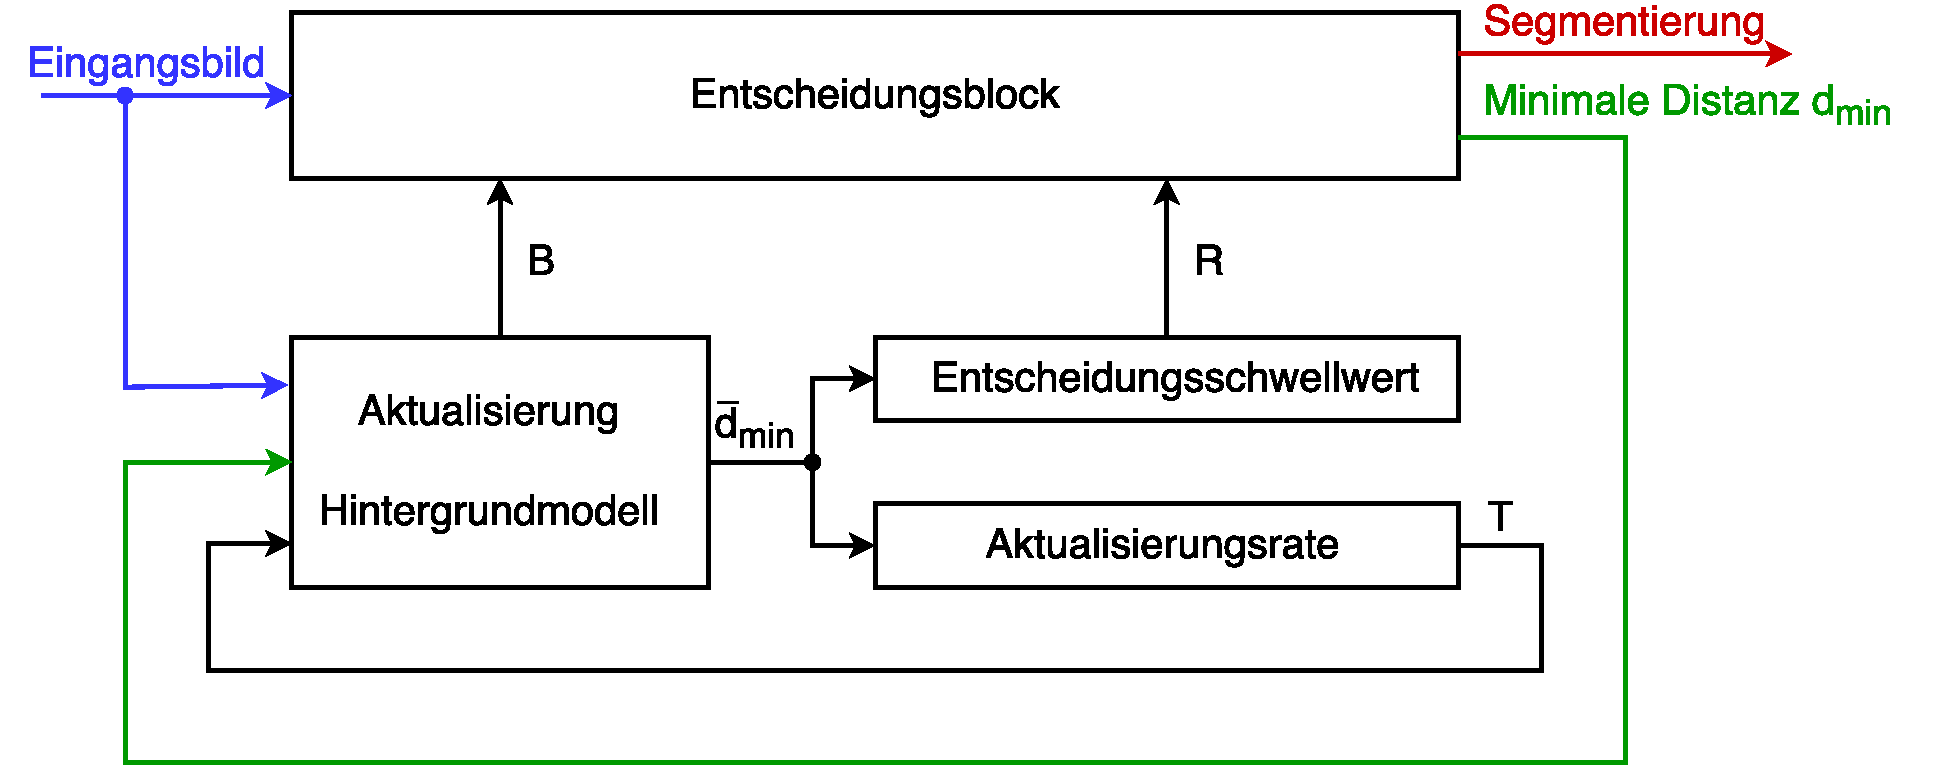
\includegraphics[width=\linewidth]{./Bilder/PDF/PBAS_Blockdiagramm.pdf}
	\end{figure}
	\begin{center}
		Blockschaltbild der Gesamtschaltung
	\end{center}
\end{frame}

\begin{frame}{Hintergrundmodelle}
	\begin{figure}
		\centering
		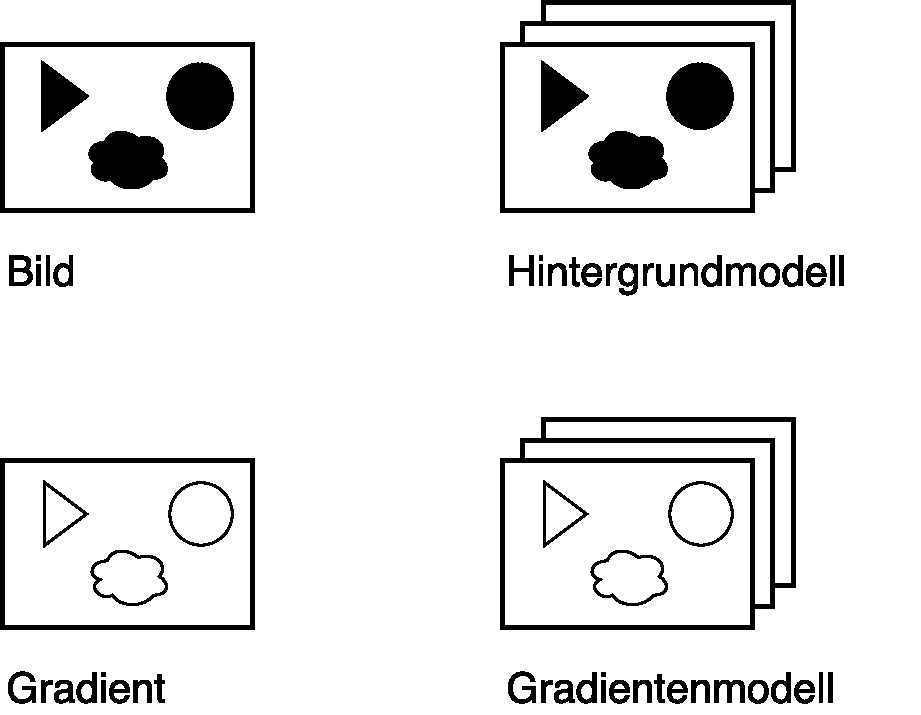
\includegraphics[width=.8\linewidth]{./Bilder/PDF/arrays.pdf}
	\end{figure}	
\end{frame}

\begin{frame}{Entscheidungsblock}
	\begin{figure}
		\centering
		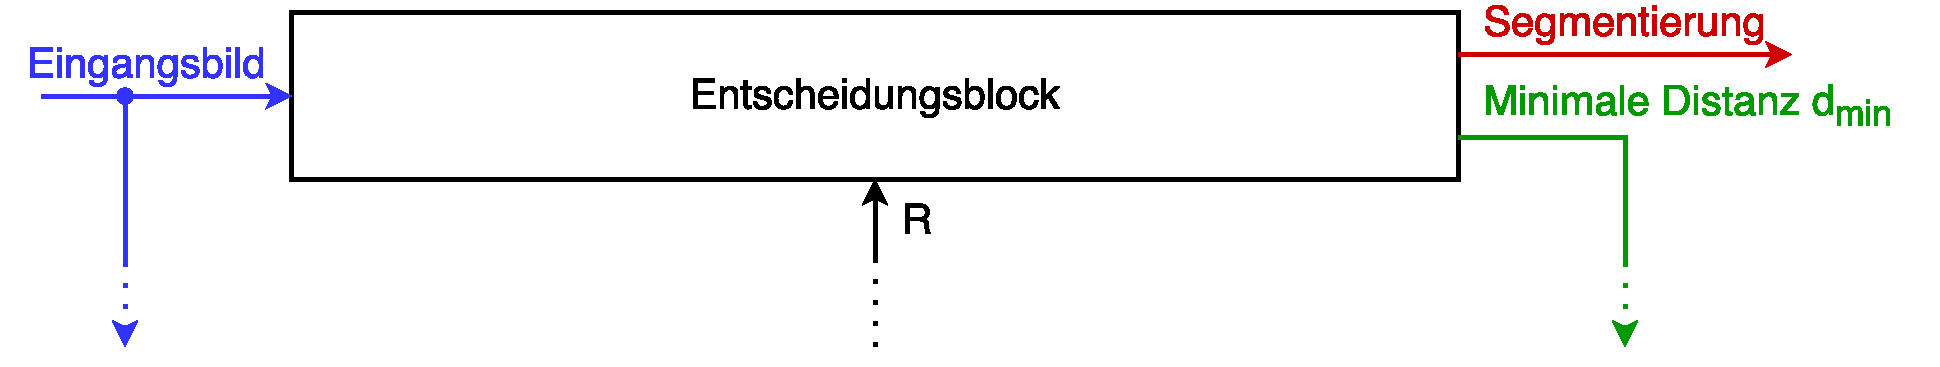
\includegraphics[width=\linewidth]{./Bilder/PDF/decision_block.pdf}
	\end{figure}

	\begin{center}
		\small
		$ Distanz = | Bild - Hintergrundmodell | + | Gradient - Gradientenmodell | $
	\end{center}
	
	\vspace{2em}
	
	$ F(x) = \left\{\begin{array}{ll} 1, & \#\left\{ Distanz < R \right\} < \#_{min} \\
				0, & sonst\end{array}\right. $
\end{frame}

\begin{frame}[t]{}

\end{frame}

\begin{frame}

\end{frame}

\begin{frame}[t]{}

\end{frame}

\end{document}
